%!TEX program = xelatex
% 完整编译: xelatex -> biber/bibtex -> xelatex -> xelatex
\documentclass[lang=cn,a4paper]{elegantpaper}
\ExecuteBibliographyOptions{sorting=none}
\title{计算机网络实验四 TCP协议的实现}
\author{彭程~~ 2020011075 \\ 清华大学~~ 自动化系~~ 自02班}
%\institute{\href{https://elegantlatex.org/}{Elegant\LaTeX{} 项目组}}

%\version{0.10}
\date{\zhtoday}

\usepackage{float}
% 本文档命令
\usepackage{array}
\newcommand{\ccr}[1]{\makecell{{\color{#1}\rule{1cm}{1cm}}}}
\addbibresource[location=local]{reference.bib} % 参考文献,不要删除
\usepackage{outlines}
\usepackage{color}



\begin{document}

\maketitle

\begin{abstract}
本文为2022秋《计算机网络及应用》实验四的实验报告。本次作业python编程实现了TCP协议。
\keywords{计算机网络,TCP}
\end{abstract}


\section{功能实现}

\noindent 本次作业实现了以下功能:

\begin{enumerate}
  \item 三次握手建立连接 (Fig.\ref{Fig.1})
  \item 双向发送小规模数据,curl www.baidu.com,获得html报文 
  \item TCP四次挥手,正确关闭 (Fig.\ref{Fig.1})
  \item 接受中等规模的数据: wget和curl均可
  \item 通过浏览器访问真实网页:百度、知乎、bilibili均可(Fig.\ref{Fig.2})
  \item 超时重传机制 (Fig.\ref{Fig.3})
  \item 缓存乱序报文等待正确报文
\end{enumerate}

\section{功能实现思路}

\subsection{构建TCP报文}
本次我使用了一个TCPPacket类,参考了\href{https://kytta.medium.com/tcp-packets-from-scratch-in-python-3a63f0cd59fe}{这里},可以实现校验和计算和构建合适的报文等功能。

\subsection{三次握手和四次挥手}

三次握手即我方发送SYN,对方回复ACK+SYN,我方回复ACK。此处app\_connnect函数第一次握手由main调用,第三次握手由tcp\_rx调用,第三次握手后tcp\_rx调用app\_connnected通知应用层。

四次挥手通常是我方接受完消息后发出FIN,对方回应ACK,对方发送FIN,我方回应ACK,之后经过等待终止连接。

\subsection{状态维护}

我维护一个全局的状态机state\_machine字典,字典的key为conn的哈希值(因此有个hash\_conn函数用来进行哈希),字典每个value为一个state类,包含seq\_num,ack\_num等必要的状态数据。这样实现了对于不同conn维护不同的状态,这对最终在浏览器打开网页有很大的帮助。

\subsection{超时重传}

我使用了提供的tick函数作为超时重传的载体,逻辑是如果是报文传递模式,如果一定时间内待发送报文的ack或者接收到报文的ack均未发生改变,则认为超时,进行重传。

\subsection{乱序报文处理}

在实验中发现报文会有乱序情况,于是对乱序报文进行处理是十分必要的。我采取的策略是,如果接受报文比需要的报文序号大,就进行缓存,当接收到需要报文时,在缓存中进行查找,若有后续报文则依次发送给应用层。




\section{收获与总结}

这次作业难度十分大,既没有往届的参考,网络上相关参考也很少。在我的不懈努力下终于较为圆满的完成了。在完成过程中当然遇到了一系列的问题:刚开始不会用wireshark对比,走了很多弯路;之后校验和算不对,又研究了半天;之后下载任务中,开始是https无法连接,之后又是传到一半会中断,最终在我使用了超时重传、乱序处理和缓存之后,终于可以保持一个较为稳定的下载(本地目前每次都可以成功)。在上传过程中一直收不到对面发来的ack,还好该任务取消了。在浏览器打开网页时一直有奇怪的连接,在我重构了状态存储机制,允许对于不同连接进行不同状态维护后,终于可以成功的用浏览器打开各种网页。

本次实验收获主要在于:对TCP的细节认识更清楚了,学会了wireshark这一重要工具,对网络中可能存在的各种问题有了更多的认识(重传、丢包等)。超时重传和缓存机制是我认为本是实验中的亮点。



\section{建议}

\noindent 以下是一些小小的建议:

\begin{enumerate}
  \item 时间有些紧张。本次考完试后突然通知于一周内完成改实验,我从周二开始做,到周六下午基本完成,每天都做5-6h,总共应该超过20h。同期还有数图大作业、科研等任务,导致这一周十分紧张,打乱了一些原有计划。建议以后在布置该项作业时,告知大家预计耗时并适当的延长完成周期。
  \item 不可知错误太多。这次作业最大的感受就是“卡”,经常在一个错误卡主,然后几个小时毫无进展,让同学们试错和提升自主解决问题的能力是可以理解的,毕竟在科研中没有人能一直帮你解决问题,但试错成本可以略微降低一点(尤其对于一个在总评中占比并不算高的作业,这个任务量和其他课的一些大作业不相上下),希望在文档中对容易出问题的地方进行更多的提示,对共性问题提供一些总结。
\end{enumerate}


\noindent 同时完全可以感受到本实验开发和答疑工作量真的很大,感谢助教提供了丰富的接口、详细的文档和耐心的答疑指导。希望以上意见对助教有所帮助。


\section*{附图}

\begin{figure}[H]
  \centering
  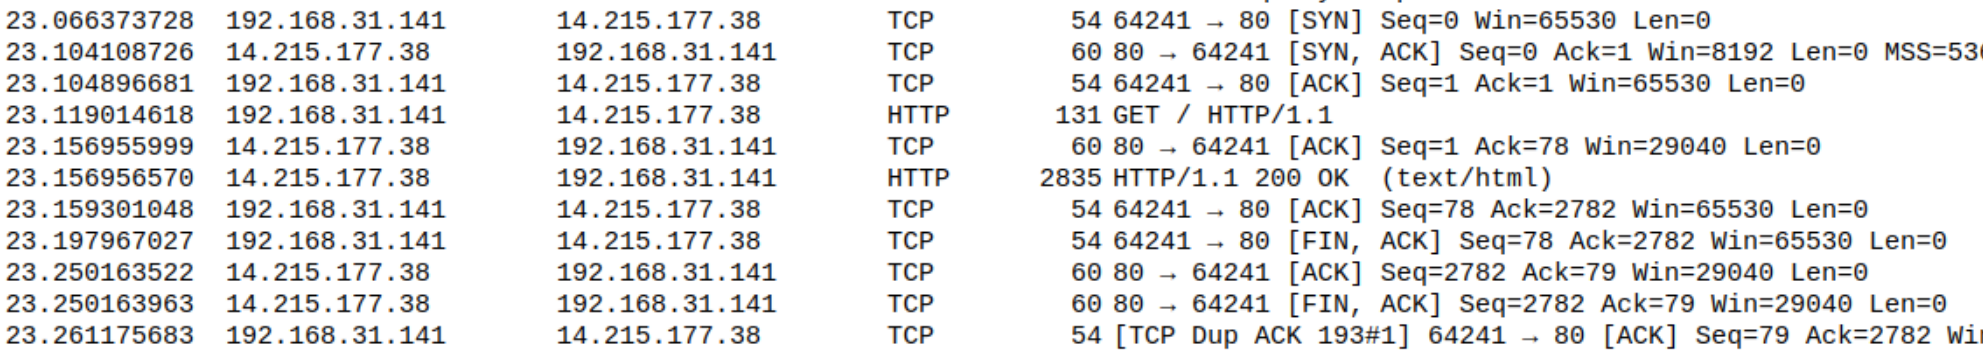
\includegraphics[width=1\textwidth]{baidu.png}
  \caption{三次握手和四次挥手} 
  \label{Fig.1}
\end{figure}

\begin{figure}[H]
  \centering
  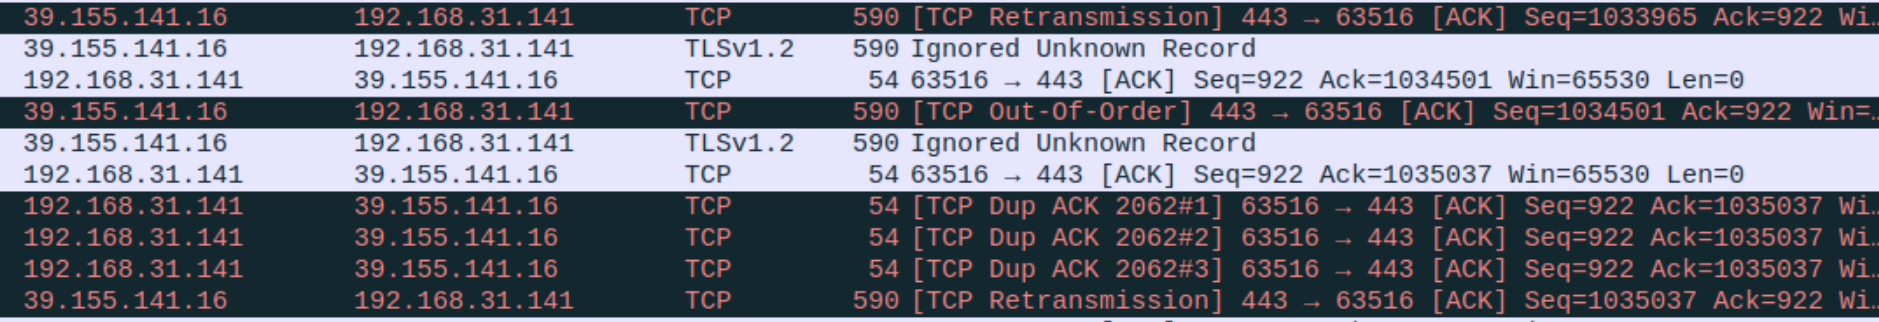
\includegraphics[width=1\textwidth]{resend.png}
  \caption{超时重传} 
  \label{Fig.2}
\end{figure}

\begin{figure}[H]
  \centering
  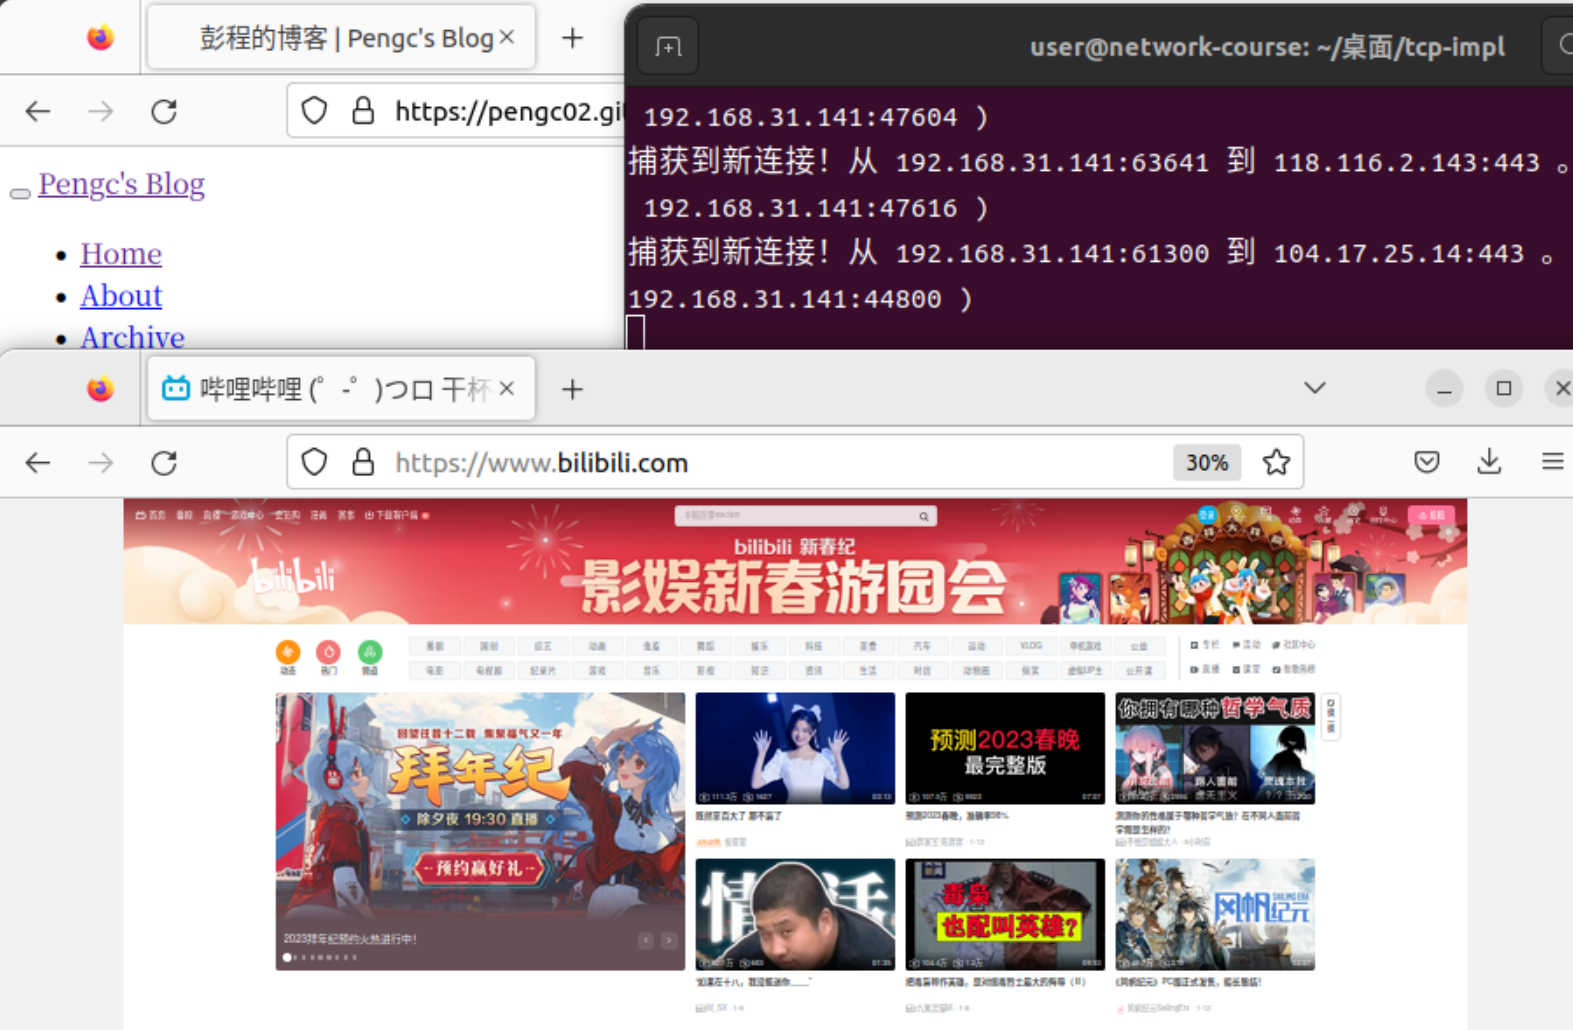
\includegraphics[width=1\textwidth]{web.png}
  \caption{浏览器打开网页} 
  \label{Fig.3}
\end{figure}


\nocite{*}
\printbibliography[heading=bibintoc, title=\ebibname]

\appendix
%\appendixpage
\addappheadtotoc

\end{document}
